%----------------------------------------------------------------------------------------
%	Graph Theory Chapter
%----------------------------------------------------------------------------------------
\chapterimage{ChapterCover.pdf} % Chapter heading image
\chapter{Graph Theory}

\epigraph{\textit{Geometric diagrams are to geometers what board and pieces are to chessmasters: visual aids, helpful but not indispensable.}}{\rightline{{\rm --- \href{https://store.doverpublications.com/products/9780486678702}{Richard J. Trudeau}}}}

\minitoc
\newpage
\section{Introduction to Graph Theory}
\subsection*{Historical Significance}
Graph theory's origins can be traced to 1736 when Leonhard Euler solved the famous Seven Bridges of K\"{o}nigsberg problem, marking the first formal proof in the field. By abstracting the physical layout of bridges and landmasses into vertices and edges, Euler created a new mathematical approach that would eventually revolutionize how we analyze networks and relationships. While the field developed slowly at first, it gained significant momentum in the 19th century when mathematicians like Arthur Cayley connected it to chemical compositions and James Joseph Sylvester introduced the term "graph" in 1878. The publication of the first textbook on graph theory by D\'enes K\H{o}nig in 1936 officially established it as a distinct branch of mathematics6. Today, graph theory serves as a cornerstone for solving complex problems across diverse fields, from computer science and biology to sociology and transportation networks5, demonstrating how a solution to a recreational puzzle evolved into a fundamental mathematical framework for understanding and optimizing interconnected systems.
 
\subsection*{Overview}
Today, graph theory provides a mathematical framework for analyzing networks of interconnected entities, where nodes (also called vertices) represent discrete objects and edges represent the relationships between them. A graph G is formally defined as an ordered pair $G = (V,E)$, where $V$ is a set of vertices and $E$ is a set of edges connecting pairs of vertices. Graphs can be categorized into several fundamental types based on their edge properties. In \gls{undirected graphs}, edges represent bidirectional relationships, such as friendship connections in social networks or pedestrian paths that can be traversed in both directions. \gls{Directed graphs} (digraphs) contain edges with specific orientations, indicating one-way relationships like hyperlinks between web pages or parent-child relationships. Additionally, graphs can be weighted, where edges carry numerical values representing costs, distances, or strengths of relationships, or unweighted, where all connections are considered equal.
\begin{wrapfigure}{R}{0.58\textwidth}
\begin{tcolorbox}[every float=\centering, drop shadow, title=Concepts of Graph Theory ,colback=white,colframe=WMgreen,
  colbacktitle=WMgreen,]
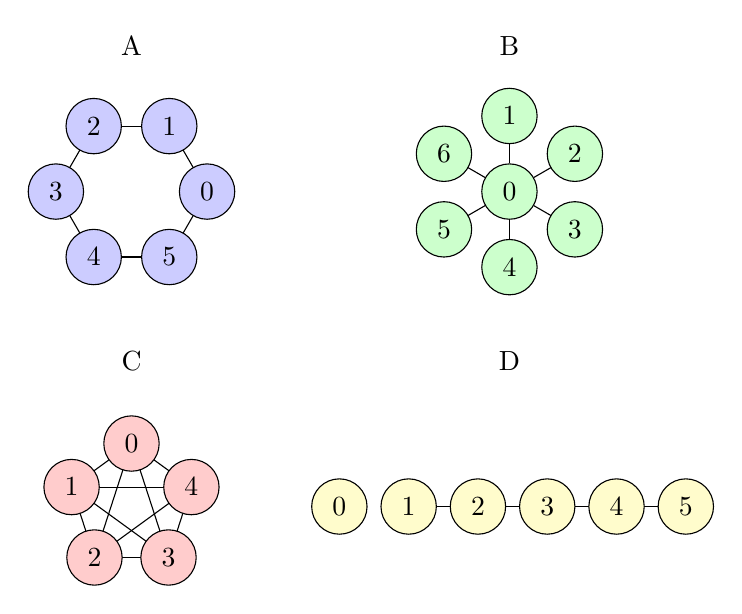
\begin{tikzpicture}[scale=0.8]
    % Define styles for nodes and edges
    \tikzstyle{vertex}=[circle,draw,minimum size=20pt,inner sep=0pt]
    
    % Graph 1: Degree (Regular Hexagon)
    \begin{scope}[shift={(-3,4)}]
        \node[above] at (0,2) {A};
        % Connect hexagon edges
        \foreach \angle in {0,60,120,180,240,300}{
            \pgfmathsetmacro{\nextangle}{\angle + 60}
            \draw (\angle:1.2) -- (\nextangle:1.2);
        }
        % Create regular hexagon vertices
        \foreach \angle/\name in {0/0, 60/1, 120/2, 180/3, 240/4, 300/5}{
            \node[vertex,fill=blue!20] at (\angle:1.2) {\name};
        }
    \end{scope}
    
    % Graph 2: Centrality (Star Graph - more evenly spaced)
    \begin{scope}[shift={(3,4)}]
        \node[above] at (0,2) {B};
        \node[vertex,fill=green!20] (c) at (0,0) {0};
        \foreach \angle/\name in {90/1, 30/2, -30/3, -90/4, -150/5, 150/6}{
            \draw (c) -- (\angle:1.2);
            \node[vertex,fill=green!20] at (\angle:1.2) {\name};
        }
    \end{scope}
    
    % Graph 3: Clustering Coefficient (Complete Graph - more symmetric)
    \begin{scope}[shift={(-3,-1)}]
        \node[above] at (0,2) {C};
        % Draw all possible edges between vertices
        \foreach \i in {0,...,4}{
            \foreach \j in {\i,...,4}{
                \ifnum\i<\j
                    \draw (\i*72+90:1) -- (\j*72+90:1);
                \fi
            }
        }
        \foreach \angle/\name in {90/0, 162/1, 234/2, 306/3, 18/4}{
            \node[vertex,fill=red!20] at (\angle:1) {\name};
        }
    \end{scope}
    
    % Graph 4: Shortest Path (Linear Path)
    \begin{scope}[shift={(3,-1)}]
        \node[above] at (0,2) {D};
        \foreach \x in {0,...,4}{
            \pgfmathsetmacro{\nextx}{\x + 1}
            \draw (\x*0.8-2,0) -- (\nextx*1.1-2.7,0);
        }
        \foreach \x in {0,...,5}{
            \node[vertex,fill=yellow!20] at (\x*1.1-2.7,0) {\x};
        }
    \end{scope}
\end{tikzpicture}
 \captionof{figure}{Graph theory concepts illustrated: (A) The cycle graph demonstrates degree, where each vertex has exactly two connections, showing uniform degree distribution. (B) The star graph highlights centrality, with node 0 having maximum centrality as it connects to all other nodes. (C) The hexagon graph shows maximum clustering coefficient, where all possible connections between neighbors exist. (D) The path graph illustrates shortest path concepts, where the distance between any two nodes is the minimum number of edges that must be traversed.}
  \label{fig:BasicGraphs}
 \end{tcolorbox}
 \end{wrapfigure}
 \FloatBarrier % Fix floating issues
 
Several key metrics help characterize graph structure and identify important network features. \gls{Degree} measures the number of connections a node has, while \gls{centrality} metrics like betweenness and closeness identify nodes that are crucial for network flow or information spread. The \gls{clustering coefficient} quantifies how tightly connected groups of nodes are, with values ranging from 0 (no clustering) to 1 (complete clustering). This measure is particularly important in social networks, where nodes tend to form dense local communities. The shortest path length between nodes helps evaluate network efficiency and can be used to identify optimal routes through the network, making it essential for applications in transportation and communication systems.

These fundamental concepts of graph theory find applications across diverse fields, from analyzing social media networks and optimizing transportation systems to modeling biological networks and designing computer algorithms. The versatility of graph theory as an analytical tool stems from its ability to represent and quantify complex relationships in a mathematically rigorous yet intuitively understandable way.

\subsection*{Applications of Graph Theory in Neuroscience}
In neuroscience, brain networks are represented as graphs where nodes typically represent brain regions, electrodes, or voxels, while edges represent structural or functional connections between these elements. This abstraction allows researchers to quantify and analyze the organizational principles of neural systems at multiple scales, from microscopic neural circuits to macroscopic brain regions.

In structural connectivity analysis, diffusion MRI data is used to construct graphs where edges represent physical white matter connections between brain regions. These structural networks provide insights into the anatomical architecture of the brain, revealing important organizational principles such as the presence of highly connected hub regions and hierarchical modular structure. Graph metrics like clustering coefficient and path length help characterize the efficiency of information transfer through these anatomical networks, while centrality measures identify critical brain regions that serve as important relay stations for neural communication.

Functional connectivity studies, whether using fMRI or EEG data, create graphs based on statistical dependencies between neural signals recorded from different brain areas. In EEG studies, for example, electrodes serve as nodes while edges represent measures of synchronization or coherence between electrode signals. These functional networks are dynamic, changing with cognitive states and tasks, and can reveal how different brain regions coordinate their activity during various cognitive processes. Graph theoretical analyses of these networks have revealed important properties like small-world organization, which balances efficient global communication with robust local processing, and hub regions that play crucial roles in integrating information across different functional modules.

Recent advances in the field have moved beyond static network analyses to study dynamic changes in graph properties over time, particularly in EEG and MEG studies where temporal resolution is high. These dynamic network analyses have revealed how brain network organization flexibly adapts to changing cognitive demands and how disruptions in these dynamic patterns may relate to various neurological and psychiatric conditions. The application of graph theory to neuroscience has thus provided not only powerful analytical tools but also new conceptual frameworks for understanding how the brain's structural and functional organization supports cognitive function.

\subsection*{Applications of Graph Theory in Psychology}
Graph theory also provides powerful analytical tools for understanding psychological and social phenomena across multiple scales. In the clinical domain, graph theory enables the construction of symptom networks where nodes represent individual symptoms and edges represent their interactions or correlations. This network approach has transformed how we conceptualize mental disorders - rather than viewing them as underlying diseases that cause symptoms, we can analyze them as systems of interacting symptoms. For instance, in depression, insomnia might lead to fatigue, which leads to reduced activity, which in turn reinforces depressive thoughts. By identifying central symptoms that trigger cascading effects, clinicians can target interventions more effectively.

Graph theoretical approaches also inform treatment planning and monitoring. By tracking changes in symptom networks over time, clinicians can assess treatment effectiveness and identify early warning signs of relapse. This dynamic network perspective helps explain why some symptoms are more resistant to treatment than others and why targeting certain symptoms might have cascading beneficial effects throughout the network. The ability to quantify network properties like centrality and clustering has provided new metrics for assessing therapeutic progress and predicting treatment outcomes.
These applications demonstrate how graph theory has evolved from a mathematical framework into an essential tool for understanding human behavior and mental health, providing both theoretical insights and practical clinical applications.

In social psychology, graph theory has become instrumental in analyzing group dynamics and social networks. Researchers use these methods to map relationships between individuals (nodes) and their social connections (edges), revealing important patterns in human interaction. This approach has helped identify how information spreads through social networks, how opinion leaders emerge, and how social support structures function. Social network analysis has revealed important principles about group formation, social influence, and community structure that weren't visible through traditional research methods.

\section{Conducting Graph Theoretical Analyses}
Network data suitable for graph theory analysis can come from many sources, including social connections, neural recordings, communication patterns, or any system with discrete elements that interact. The key is identifying meaningful nodes (the elements) and edges (their relationships). For example, in EEG data, nodes might be electrodes while edges represent functional connectivity between brain regions. Data are typically organized into an adjacency matrix (showing which nodes connect to each other) but can also be organized into an edge list (explicitly listing all connections).

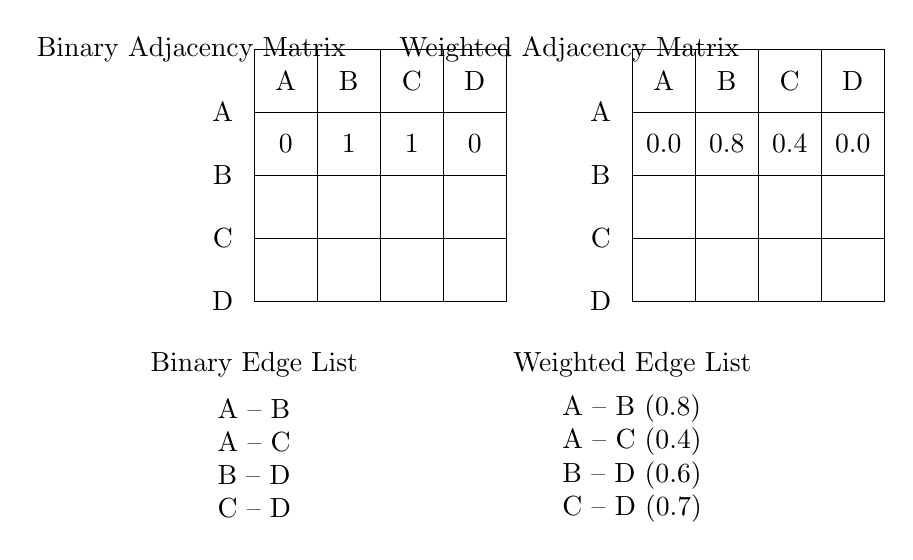
\begin{tikzpicture}[scale=0.8]
    % Binary Adjacency Matrix
    \begin{scope}[shift={(-6,0)}]
        \node at (-1,4) {Binary Adjacency Matrix};
        
        % Draw matrix grid
        \foreach \x in {0,1,2,3} {
            \foreach \y in {0,1,2,3} {
                \draw (\x,\y) rectangle (\x+1,\y+1);
            }
        }
        
        % Add labels
        \foreach \x/\l in {0/A,1/B,2/C,3/D} {
            \node at (\x+0.5,3.5) {\l};
            \node at (-0.5,3-\x) {\l};
        }
        
        % Fill in binary values (0/1)
        \node at (0.5,2.5) {0};
        \node at (1.5,2.5) {1};
        \node at (2.5,2.5) {1};
        \node at (3.5,2.5) {0};
    \end{scope}
    
    % Weighted Adjacency Matrix
    \begin{scope}[shift={(0,0)}]
        \node at (-1,4) {Weighted Adjacency Matrix};
        
        % Draw matrix grid
        \foreach \x in {0,1,2,3} {
            \foreach \y in {0,1,2,3} {
                \draw (\x,\y) rectangle (\x+1,\y+1);
            }
        }
        
        % Add labels
        \foreach \x/\l in {0/A,1/B,2/C,3/D} {
            \node at (\x+0.5,3.5) {\l};
            \node at (-0.5,3-\x) {\l};
        }
        
        % Fill in weighted values
        \node at (0.5,2.5) {0.0};
        \node at (1.5,2.5) {0.8};
        \node at (2.5,2.5) {0.4};
        \node at (3.5,2.5) {0.0};
    \end{scope}
    
    % Binary Edge List
    \begin{scope}[shift={(-6,-5)}]
        \node at (0,4) {Binary Edge List};
        
        \node[align=left] at (0,2.5) {
            A -- B \\
            A -- C \\
            B -- D \\
            C -- D
        };
    \end{scope}
    
    % Weighted Edge List
    \begin{scope}[shift={(0,-5)}]
        \node at (0,4) {Weighted Edge List};
        
        \node[align=left] at (0,2.5) {
            A -- B (0.8) \\
            A -- C (0.4) \\
            B -- D (0.6) \\
            C -- D (0.7)
        };
    \end{scope}
\end{tikzpicture}

In EEG research, each electrode recording brain activity serves as a node in the network. The relationships between these nodes are quantified through various measures of functional connectivity. These connections can be measured through phase locking values, which capture the consistency of phase relationships between signals from different electrodes, correlation coefficients that measure the linear relationship between electrode signals, or more sophisticated measures like Granger causality that assess directional influences between brain regions. This approach allows researchers to understand how different brain regions communicate and coordinate during various cognitive tasks or states.

In clinical settings, network analysis provides a framework for understanding how psychological symptoms interact and influence each other. Nodes in these networks represent individual symptoms or psychological variables, while edges capture their relationships. These relationships can be established through various means: symptoms that frequently co-occur, patients' reports of how one symptom influences another, or patterns observed over time in longitudinal studies. This approach has revolutionized our understanding of mental disorders, moving from a disease model to viewing psychological disorders as systems of interacting symptoms.

Social psychology utilizes network analysis to understand human relationships and group dynamics. In these networks, nodes typically represent individuals or social entities (like groups or organizations), while edges represent various types of social relationships. These connections can represent direct communication patterns, friendship ties, or shared group memberships. The strength of these relationships can be represented either as binary connections (present/absent) or weighted edges that indicate the intensity or frequency of interaction. This framework helps researchers understand social influence, group formation, and information flow within communities.

\subsection*{Data Processing Steps}
Before analysis, several preprocessing steps are crucial. First, check for missing or impossible connections in your network data. Consider whether to include weighted edges (showing connection strength) or just binary connections. Think carefully about thresholding - deciding how strong a relationship must be to count as an edge. For time-series data like EEG, you'll need to address noise and artifacts that could create spurious connections. It's also important to consider whether your network should be directed (connections have a specific direction) or undirected.

Your adjacency matrix should be sparse. A sparse matrix is one in which most elements are zero, with only a small percentage of non-zero entries. In graph theoretical analysis, sparse matrices are crucial because they better reflect real-world networks where nodes typically connect to only a small subset of other nodes rather than everything connecting to everything else. Using sparse matrices provides several key advantages, requiring less computational resources and memory for storage and processing, enabling faster algorithm execution, and often better representing natural phenomena like neural networks where excessive connectivity would be energetically costly and potentially noisy. In neuroscience specifically, sparse connectivity helps support efficient information processing by promoting better pattern separation and more effective stimulus encoding. The sparsity principle is particularly important when analyzing large-scale networks, as it helps maintain computational tractability while preserving the most meaningful connections in the network.


Thresholding is a crucial step in creating sparse networks from correlation matrices for graph theoretical analysis. This process involves making deliberate choices about which connections to maintain and which to eliminate, ultimately creating a more meaningful and computationally manageable network structure.
The first step involves selecting a threshold value to determine which correlations are strong enough to be considered meaningful connections. This threshold might be based on statistical significance (e.g., p-values), correlation strength (e.g., keeping only correlations above 0.3 or 0.5), or proportional thresholding (keeping the top percentage of strongest connections). Connections falling below this threshold are set to zero, effectively removing weak or potentially spurious relationships from the network. This step is crucial because weak correlations may represent noise rather than true functional relationships.

The next step involves removing self-correlations by setting the diagonal elements of the matrix to zero. Self-correlations (correlations of a node with itself) are always 1.0 and don't provide meaningful information about network structure. After thresholding and removing self-correlations, researchers must decide whether to maintain the weighted edges (keeping the actual correlation values) or convert to binary connections (where any surviving connection is set to 1). Binary networks are simpler to analyze and interpret, but weighted networks preserve more detailed information about connection strengths. This choice should be guided by the research questions and the specific requirements of the analysis methods being used.

The resulting sparse network retains only the most meaningful connections while eliminating potentially spurious relationships, making it both more interpretable and computationally tractable. This process is particularly important when analyzing large networks, as it helps focus the analysis on the most robust and meaningful patterns in the data.

\subsection*{Analysis Methods}
Start analysis with basic graph metrics like degree (number of connections per node), clustering coefficient (how interconnected neighboring nodes are), and various centrality measures (identifying important nodes). These graph metrics provide essential tools for quantifying and understanding network properties.  

\subsubsection*{Clustering Coefficient}
The clustering coefficient measures how much nodes tend to cluster together in a network. There are two versions of clustering  coefficient; the global and the local. The global coefficient gives an overall indication of the clustering in the network, whereas the local coefficient gives an indication of the embeddedness of single nodes within a cluster. 

The global clustering coefficient is based on triplets of nodes. A triplet consists of three connected nodes. A triangle therefore includes three closed triplets, one centered on each of the nodes (n.b. this means the three triplets in a triangle come from overlapping selections of nodes). The global clustering coefficient is the number of closed triplets (or 3 x triangles) over the total number of triplets (both open and closed). The first attempt to measure it was made by Luce and Perry (1949). This measure gives an indication of the clustering in the whole network (global), and can be applied to both undirected and directed networks. 

Before delving into the local clustering coefficient, let's formalize the definition of the components of a graph. A graph $G=(V,E)$ formally consists of a set of vertices $V$ (nodes) and a set of edges $E$ between them. An edge $e_{ij}$ connects vertex $v_{i}$  with vertex $v_{j}$. The neighborhood $N_{i}$ for a vertex $v_{i}$ is defined as its immediately connected neighbors as follows: $N_i = \{v_j : e_{ij} \in E \lor e_{ji} \in E\}$. In simpler terms, the neighborhood $N_i$ is the set of vertices j such that there is an edge from node $i$ to node $j$ or from node $j$ to node $i$ in the set of all edges $E$.

For a directed graph, $e_{ij}$ is distinct from $e_{ji}$, and therefore for each neighborhood $N_{i}$ there are $k_{i}(k_{i}-1)$ links that could exist among the vertices within the neighborhood ($k_{i}$ is the number of neighbors of a vertex). Thus, the local clustering coefficient for directed graphs is given as $C_{i}={\frac {|\{e_{jk}:v_{j},v_{k}\in N_{i},e_{{jk}}\in E\}|}{k_{i}(k_{i}-1)}}$. 

An undirected graph has the property that $e_{ij}$ and $e_{ji}$ are considered identical. Therefore, if a vertex $v_{i}$ has $k_{i}$ neighbors, $\frac {k_{i}(k_{i}-1)}{2}$   edges could exist among the vertices within the neighborhood. Thus, the local clustering coefficient for undirected graphs can be defined as $C_{i}=\frac {2|\{e_{{jk}}:v_{j},v_{k}\in N_{i},e_{{jk}}\in E\}|}{k_{i}(k_{i}-1)}$.   


%Now, let's define k_{i}    as the number of vertices, |N_{i}|    , in the neighborhood, N_{i}    , of a vertex. The local clustering coefficient C_{i}    for a vertexv_{i}    is then given by the proportion of links between the vertices within its neighborhood divided by the number of links that could possibly exist between them. For a directed graph, e_{ij}    is distinct from e_{{ji}}    , and therefore for each neighborhood N_{i}    there are k_{i}(k_{i}-1)    links that could exist among the vertices within the neighborhood ( k_{i}    is the number of neighbors of a vertex). Thus, the local clustering coefficient for directed graphs is given as [2] C_{i}={\frac {|\{e_{{jk}}:v_{j},v_{k}\in N_{i},e_{{jk}}\in E\}|}{k_{i}(k_{i}-1)}}    . 

%For a given node, it is calculated as the proportion of actual connections between its neighbors divided by all possible connections between them. Mathematically, for a node $i$ with $k_i$ neighbors, the clustering coefficient $C_i = (2 × L_i)/(k_i × (k_i-1))$, where $L_i$ is the number of links between the $k_i$ neighbors. The global clustering coefficient is the average of all local coefficients, indicating overall network clustering.

\begin{figure}[h]
\centering
\begin{tcolorbox}[halign=center,  % Centers content horizontally within tcolorbox
    every float=\centering,
    drop shadow,
    title=The Clustering Coefficient,
    colback=white,
    colframe=WMgreen,
    colbacktitle=WMgreen]
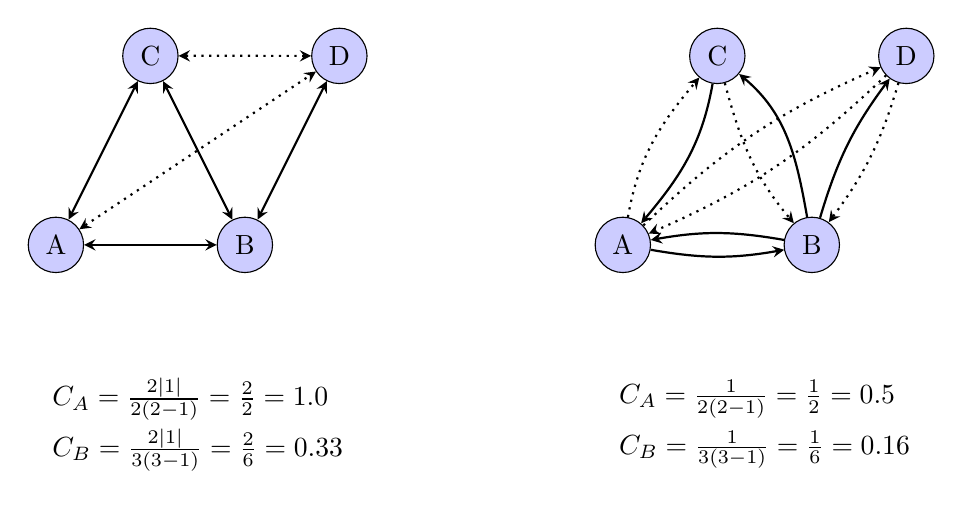
\begin{tikzpicture}[scale=1.2,baseline=(current bounding box.center)]
    % Define styles
    \tikzstyle{vertex}=[circle,draw,fill=blue!20,minimum size=20pt,inner sep=0pt]
    \tikzstyle{biduredge}=[thick,<->,>=stealth]
    \tikzstyle{inedge}=[thick,<-,>=stealth]
    \tikzstyle{outedge}=[thick,->,>=stealth]
    \tikzstyle{possibleedge}=[thick,<->,>=stealth,dotted]
    \tikzstyle{possibledir}=[thick,dotted,->,>=stealth]
    
    %Draw the non-directed graph
    % Draw the nodes
    \node[vertex] (1) at (1,0) {A};
    \node[vertex] (2) at (3,0) {B};
    \node[vertex] (3) at (2,2) {C};
    \node[vertex] (4) at (4,2) {D};
    
    % Draw the edges
    \draw[biduredge] (1) -- (2);
    \draw[biduredge] (1) -- (3);
    \draw[biduredge] (2) -- (3);
    \draw[biduredge] (2) -- (4);
    \draw[possibleedge] (3) -- (4);
    \draw[possibleedge] (1) -- (4);
    
    % Add calculation explanation
    \node[align=left] at (2.5,-2) {
        $C_A = \frac{2 |1|}{2(2-1)} = \frac{2}{2} = 1.0 $\\
        %\footnotesize{\emph{(All of A's neighbors (B and C) are connected)}} \\
        \vspace{-.2cm}\\
        $C_B = \frac{2|1|}{3(3-1)} = \frac{2}{6} = 0.33$ \\
        %\footnotesize{\emph{(Only 1 connection exists between}}\\
        %\footnotesize{\emph{two of B's neighbors when three connections are possible)}}
    };
    
    %Draw the directed graph
    % Draw the nodes
    \node[vertex] (5) at (7,0) {A};
    \node[vertex] (6) at (9,0) {B};
    \node[vertex] (7) at (8,2) {C};
    \node[vertex] (8) at (10,2) {D};
    
    % Draw the edges
    \draw[inedge] (5) to[out=10,in=170] (6);
    \draw[inedge] (6) to[out=-170,in=-10] (5);
    \draw[inedge] (5) to[out=50,in=260] (7);
    \draw[possibledir] (5) to[out=80,in=230] (7);
    \draw[outedge] (6) to[out=100,in=320] (7);
    \draw[possibledir] (7) to[out=285,in=130] (6);
    \draw[outedge] (6) to[bend left=10] (8);
    \draw[possibledir] (8) to[bend right=-10] (6);
    \draw[possibledir] (5) to[bend left=10] (8);
    \draw[possibledir] (8) to[bend right=-10] (5);
    
    % Add calculation explanation
    \node[align=left] at (8.5,-2) {
        $C_A = \frac{1}{2(2-1)}= \frac{1}{2} = 0.5 $\\
       % \footnotesize{\emph{(Only 1 of two possible connections between neighbors B and C)}} \\
          \vspace{-.2cm}\\
        $C_B = \frac{1}{3(3-1)} = \frac{1}{6} = 0.16$ \\
        %\footnotesize{\emph{(Only 1 connection exists when}}\\
        %\footnotesize{\emph{6 are possible possible between its neighbors)}}
    };    
\end{tikzpicture}
  \captionof{figure}{Calculating the clustering coefficient for directed and undirected graphs.}
  \label{fig:clustercoeff}
 \end{tcolorbox}
\end{figure}

\subsubsection*{Path Length}
Path length measures the efficiency of information flow through the network. The shortest path length between two nodes is the minimum number of edges that must be traversed to get from one node to another. The characteristic path length of a network is the average shortest path length between all possible pairs of nodes. In weighted networks, path lengths consider edge weights, where stronger connections (higher weights) typically represent shorter effective distances.
Centrality Measures
Centrality identifies influential nodes using several metrics:
Degree centrality: Simply counts the number of connections a node has
Betweenness centrality: Measures how often a node lies on shortest paths between other nodes
Closeness centrality: Calculates how close a node is to all other nodes in the network
Eigenvector centrality: Considers both the quantity and quality of connections, where connections to high-scoring nodes contribute more
Community Detection
Community detection algorithms identify groups of nodes that are more densely connected to each other than to the rest of the network. Common approaches include:
Modularity optimization: Maximizes the difference between actual and expected connections within communities
Hierarchical clustering: Groups nodes based on similarity or connection strength
Spectral clustering: Uses eigenvalues of the network's adjacency matrix to partition nodes into communities
These metrics together provide a comprehensive characterization of network structure and organization, revealing important patterns in complex systems.



More advanced analyses might examine community structure, path lengths between nodes, or network efficiency. Always validate your results against null models to ensure findings are meaningful. Visualization tools can help interpret results - consider force-directed layouts for small networks or matrix representations for larger ones.
Practical Implementation
Begin with simple examples where students can calculate metrics by hand to build intuition. Then progress to using established software packages like NetworkX (Python) or igraph (R) for larger analyses. Emphasize the importance of understanding what each metric means in the context of your specific data. For instance, high clustering in social networks might indicate tight-knit communities, while in neural networks it might suggest efficient local processing.
Remember that graph theory is just a tool - the key is using it to answer meaningful questions about your system of interest. Start simple and gradually build complexity as students gain confidence with the concepts and techniques.
